%!TEX TS-program = xelatex

\documentclass[a4paper]{article}

\usepackage[english]{babel}   %% загружает пакет многоязыковой вёрстки
\usepackage{fontspec}      %% подготавливает загрузку шрифтов Open Type, True Type и др.
%\defaultfontfeatures{Ligatures={TeX},Renderer=Basic}  %% свойства шрифтов по умолчанию
\setmainfont[Ligatures={TeX},
	SmallCapsFont={Brill},
	SmallCapsFeatures={Letters=SmallCaps}]{Brill} %% задаёт основной шрифт документа
\usepackage{indentfirst}

%%% Дополнительная работа с математикой
\usepackage{amsmath,amsfonts,amssymb,amsthm,mathtools} % AMS
\usepackage{icomma} % "Умная" запятая: $0,2$ --- число, $0, 2$ --- перечисление

%%% Работа с картинками
\usepackage{wrapfig} % Обтекание рисунков текстом
\usepackage{subcaption}
\usepackage{rotating}
\usepackage{hhline}
\usepackage{lscape}
\usepackage[usenames,dvipsnames,svgnames,table,rgb]{xcolor}%пакет для использования цветов 

\usepackage{enumitem}
\setlist{nolistsep, leftmargin=5mm}

%%% Работа с таблицами
\usepackage{array,tabularx,tabulary,booktabs} % Дополнительная работа с таблицами
\usepackage{longtable}  % Длинные таблицы
\usepackage{multirow} % Слияние строк в таблице

\usepackage{multicol} % Несколько колонок

%%% Страница
\usepackage{geometry} % Простой способ задавать поля
	\geometry{top=12mm}
	\geometry{bottom=23mm}
	\geometry{left=23mm}
	\geometry{right=19mm}

%\usepackage{fancyhdr} % Колонтитулы
% 	\pagestyle{fancy}
 	%\renewcommand{\headrulewidth}{0pt}  % Толщина линейки, отчеркивающей верхний колонтитул
% 	\lfoot{Нижний левый}
% 	\rfoot{Нижний правый}
% 	\rhead{Верхний правый}
% 	\chead{Верхний в центре}
% 	\lhead{Верхний левый}
%	\cfoot{Нижний в центре} % По умолчанию здесь номер страницы

\usepackage{setspace} % Интерлиньяж
%\onehalfspacing % Интерлиньяж 1.5
\doublespacing % Интерлиньяж 2
%\singlespacing % Интерлиньяж 1

\usepackage{lastpage} % Узнать, сколько всего страниц в документе.
\usepackage{soul} % Модификаторы начертания
\usepackage{hyperref}
\usepackage[usenames,dvipsnames,svgnames,table,rgb]{xcolor}
\hypersetup{				% Гиперссылки
    colorlinks=true,       	% false: ссылки в рамках; true: цветные ссылки
    linkcolor=black,          % внутренние ссылки
    citecolor=black,        % на библиографию
    filecolor=black,      % на файлы
    urlcolor=ForestGreen          % на URL
}

\usepackage{environ}
\makeatletter
\newsavebox{\measure@tikzpicture}
\NewEnviron{scaletikzpicturetowidth}[1]{%
	\def\tikz@width{#1}%
	\def\tikzscale{1}\begin{lrbox}{\measure@tikzpicture}%
		\BODY
	\end{lrbox}%
	\pgfmathparse{#1/\wd\measure@tikzpicture}%
	\edef\tikzscale{\pgfmathresult}%
	\BODY
}
\makeatother

%%% Лингвистические пакеты
%\usepackage{savetrees} % пакет, который экономит место
\usepackage{forest} % для рисования деревьев
\usepackage{vowel} % для рисования трапеций гласных
\usepackage{natbib}
\bibpunct[: ]{(}{)}{;}{a}{}{,}

\renewcommand{\thesection}{\arabic{section}.}
\renewcommand{\thesubsection}{\arabic{section}.\arabic{subsection}}
\setlength{\columnsep}{1.6cm}

\usepackage{sectsty}
\sectionfont{\normalsize}
\subsectionfont{\normalsize}
\usepackage{titlesec}
\titlespacing*{\section}
{0pt}{2ex plus 0ex minus .2ex}{0ex plus .2ex}
\titlespacing*{\subsection}
{0pt}{2ex plus 0ex minus .2ex}{0ex plus .2ex}
\newlength{\bibitemsep}\setlength{\bibitemsep}{.2\baselineskip plus .05\baselineskip minus .05\baselineskip}
\newlength{\bibparskip}\setlength{\bibparskip}{0pt}
\let\oldthebibliography\thebibliography
\renewcommand\thebibliography[1]{%
	\oldthebibliography{#1}%
	\setlength{\parskip}{\bibitemsep}%
	\setlength{\itemsep}{\bibparskip}%
}
\begin{document}
\title{Circassians: ethnic identity and education}
\author{George Moroz \thanks{Moscow, Linguistic Convergence Laboratory, National Research University Higher School of Economics}}
\date{\vspace{-5ex}}
\maketitle

Key words: Circassians, school education, ethnic identity \bigskip

\section{Introduction}
Circassians form one of the indigenous ethnic groups of the Caucasus. After the Caucasian War a large portion of the Circassian population migrated to the Ottoman Empire, and today Circassians are settled in Russia, Turkey, Syria, Israel, Jordan, and Iraq. This article will discuss Circassians, their ethnic identity and education. We will cover the history of usage Circassian languages in education and show the current range of Circassian language education in the world. We will see that even officially declared high estimates of primary education in Circassian in Russia conceal the real picture of Circassian literacy. The results obtained during the fieldwork in multiple Circassian villages in Russia are presented with a map.

\section{Circassian ethnonym and language}
\par The Circassians are an indigenous people of the North Caucasus, where they lived until the Caucasian war (1817--1864). As a result of the war many Circassians were killed, evicted from their native lands to areas under Cossack administration, or exiled to the Ottoman Empire \citep{shenfield99, richmond13}. Today, Circassians live in Russia (mainly in the Republic of Adygea, the Karachay--Cherkessia Republic,  the Kabardino--Balkar Republic, and Krasnodar Krai), Turkey, Syria, Israel, Jordan, and Iraq.
\par The word \textit{Circassian} is an exonim that became attached to this group by the nineteenth century. The endonym used among all Circassians is Adyghe [ad'əɡɐ] or [ad'əɣɐ]. There are also traditional tribal divisions into\textit{Abdzakh}, \textit{Bzhedug},  \textit{Shapsug}, \textit{Temirgoy}, \textit{Besleney}, \textit{Kabardian} and others, that are sometimes used as andonyms. During the Soviet Union and in modern Russia Circassians lived in three separate administrative entities, and currently the exonim and endonym used for Circassians who live in the Republic of Adygea is \textit{Adygheyans}, in the Kabardino--Balkar Republic --- \textit{Kabardians}, in the Karachay--Cherkessia Republic --- \textit{Cherkessians}. Although the Kabardian language, which in the Russian tradition is called Kabardian-Cherkessian \textit{кабардино--черкесский}) is treated as the same language used by speakers from Karachay--Cherkessia and Kabardino--Balkar Republics, is treated as the same language but used by speakers from the Karachay-Cherkessia and Kabardino-Balkar Republics, some scholars recognise three different literary traditions that developed during the Soviet Union \cite[46--47]{alkhasova15}. Before the next Russian census Circassian activists are trying to apply the ethnonym \textit{Circassian} and avoid \textit{Kabardian}, \textit{Adygheyan}, and \textit{Shapsug} (since many Shapsugs live in Krasnadar Krai, they prefer to call themselves \textit{Shapsug}).
\par Circassian languages form the Northwest Caucasian language family along with the Abkhaz--Abaza branch and Ubykh. Grammatically and phonetically this language family differs significantly from other languages in the area such as Russian, Turkic, and Arabic, among others.  Circassian languages could be divided into West Circassian (Adyghe) and East Circassian (Kabardian) and these lects are traditionally treated as separate languages \citep{hewitt05}. The main West Circassian dialects are Abdzakh, Bzhedug,  Shapsug, Temirgoy, the main East Circassian dialects are Kabardian and Besleney, but in some works one can find more suffistacated division. Circassian languages show varying levels of vitality in different Circassian comunities: vitality is high in Russia (\citep{lalor88} and personal observations), Israel \citep{kreindler95}, and Jordan \citep{abdeljawad2006}, but in Turkey, for example, less than 20 percent of Circassians can still speak the Circassian languages \cite[130]{richmond13}, and in Egypt Circassian languages have suffered complete attrition \cite[53--54]{abdeljawad2006}.

\section{Circassians education}
Circassian education
First mention of Circassian education was made by Baron P. K. von Uslar in \citep{uslar87}. Von Uslar described the spread of literacy among indigenous people of the Caucasus, and proposed a school model for indigenous people of the Caucasus and a model for an alphabet for indigenous languages based on the Cyrillic alphabet. He also mentioned an alphabet created by Umar Bersey in 1855 which was used for educational purposes in the Stavropol gymnasium \cite[20]{uslar87}. There were many other orthography projects in Russia, Turkey, and Egypt \cite[12--19]{kumachova72_history}, but most of them were not used in education. The Soviet Union led a literacy campaign during the 1920s and 1930s, but because minority languages did not have government support, only in 1935 with the introduction of a new language policy were indigenous languages promoted in schools and were indigenous cultures represented on the stage. This period was cut short by the Great Terror and World War II. Later, when school education was extended in primary school, indigenous languages were still in use but Russian was used in all other educational programs. In Turkey the proccess of Turkification resulted in a descriminatory language use policy (\textit{İskan Kanunu} 1934) and education (\textit{Tehvid-i Tedrisat Kanunu} 1924), so education of, and even usage of, Circassian languages was banned until 1961, when the new Turkish Constitution was enacted. Due to the lack of literacy support from the goverment at the begining of the 20th century the overall literacy rate in Turkish in 1945 was 24.2\% and 25.6\% among the Circassian population \cite[141]{unesco53}. In the French Mandate established after World War I on the territory of present-day Syria and Lebanon, Circassian had more cultural freedom: in 1933 the first Circassian school in Quneitra was opened and briefly operated \cite[119--120]{richmond13}. Although Circassians used to have more freedom in Jordan, it was only in 1973 that the first private Circassian school was established. Circassian has not been used as a language of instruction, but only as a school subject \cite[64]{abdeljawad2006}. In Palestine after World War I the British set up a national system of education in Hebrew and Arabic and the same system was adopted by the new State of Israel, so Circassian was used only at home until the 1960s, when a Kfar Kama teacher picked up some Circassian language broadcasts from the USSR. In 1971 it was decided that in Kfar Kama Circassian would be a compulsory school subject.  From 1976 Arabic was no longer used, and Hebrew was designated as the sole language of instruction. In the other Circassian village in Israel --- Reihaniya --- primary --- and in some cases secondary --- school instruction is still Arabic, but Hebrew is taught as a compulsory school subject \cite[176-177]{stem89}.
Today, higher education programs in Circassian language and philology are available only in three universities:
\begin{itemize}
\item  \textbf{Adyghe State University} in Maykop (in Russian it is actualy called \textit{Adyghey}, \textit{Адыгейский}, and not \textit{Adyghe}, \textit{Адыгский})
\item \textbf{Kabardino-Balkar State University named after H.M. Berbekov} in Nalchik
\item \textbf{Düzce University} in Düzce 
\end{itemize}
\par From a cultural standpoint, different populations of the Circassian diaspora fared differently: some groups preserved their ethnicity, traditions, and languages, while others did not. It is clear that the various goverments showed the whole range of support stratagies: from a total lack of support to some shool and even university programs. Despite the cruel history of Russian and Soviet goverment interaction with Circassians, it could be claimed that in the republics in the Circassian homeland there is now the strongest support for the Circassian population and its language. The Russian Federal State Statistics Service identified from around 100--130 Adyghe schools and around 170--220 Kabardian schools where Circassian is taught as a school subject. Moreover, the Russian Federal State Statistics Service identified around 20--40 Adyghe schools and around 70--110 Kabardian schools where Circassian is used as a language of instruction; see Figure~\ref{fig:circ-in-school}. In the next section we will look at some issues with this data.
\begin{figure}[t]
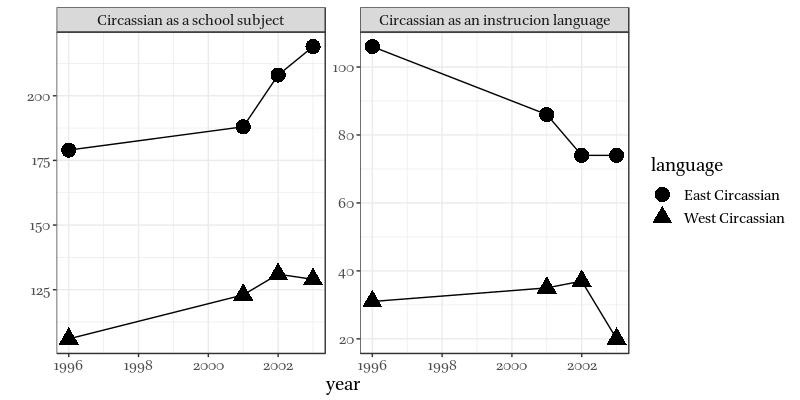
\includegraphics[width=\linewidth]{1_circassian_in_school_800_400}
\caption{Circassian languages in school education in Russia; from Russian Federal State Statistics Service, http://www.gks.ru}
\label{fig:circ-in-school}
\end{figure} 

\section{Circassian school education in Russia}
Unfortunately, the linguistic distance between different Circassian lects is not the same, and as a result some idioms are not easy to learn. There are several cases when there is linguistic distance between the standard language taught in school and the vernacular:

\begin{itemize}
\item is small (106 in total, 67\%):
\begin{itemize}
\item in ten Temirgoy and one Abdzakh villages in the Republic of Adygea,
\item in one Temirgoy village in Krasnodar Krai,
\item in fourteen villages in the Karachay--Cherkessia Republic,
\item   and eighty villages in the Kabardino--Balkar Republic
\end{itemize}
\item is large (48 in total, 30\%): 
\begin{itemize}
\item twenty eight Bzhedug, five Shapsug, three Kuban and one Besleney villages in the Republic of Adygea,
\item in eight Shapsug and one Bzhedugh vilages in Krasnodar Krai,
\item in two Besleney villages in the Karachay--Cherkessia Republic
\end{itemize}   
\item there is no school education in a village (4 in total, 2\%):
\begin{itemize}
\item in two Shapsug villages in Krasnodar Krai,
\item in one Besleney village in Krasnodar Krai,
\item in villages with Circassian population in Stavropol Krai.
\end{itemize}
\end{itemize}

\par All data about school education comes from my fieldwork completed during 2014-2018. The enumerated types are presented in Figure~\ref{fig:map} (created with R \citep{rcitation19} package \texttt{lingtypology} \citep{moroz17}).

\begin{figure}[t]
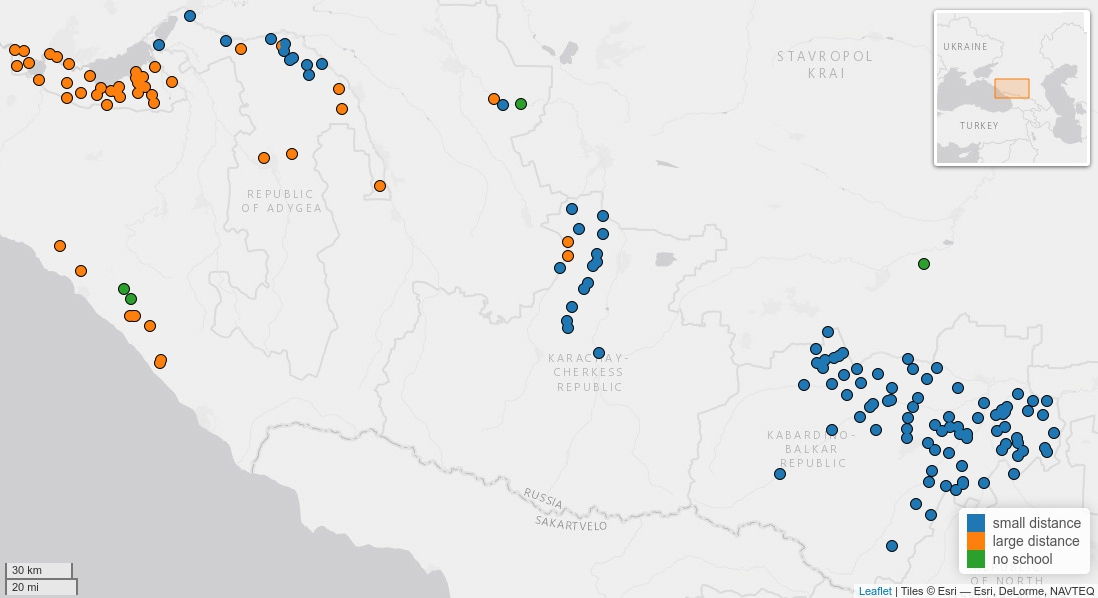
\includegraphics[width=\linewidth]{2_map_1100_600.jpeg}
\caption{Circassian villages in Russia colored by distance between language taught in school and vernacular}
\label{fig:map}
\end{figure} 

\section{Conclusion}
In this work we have reviewed important information about Circassian ethnic identity, and looked at data concerning Circassian education during the XIX--XXI centuries. It is clear that the world’s Circassian population mostly learns the language at home, and in most cases there is no goverment support for extended learning (e. g. literacy in the native language). We could find a relatively strong system of Circassian school education in Russia, but people in more than 30\% of settlements (their distribution is presented on the map, see Figure~\ref{fig:map}) were required to learn a distant dialect or even another language during these classes. So classes that were expected to support indigenous languages appear to be lessons of other foreign languages. This is not unique to Circassian settlements --- there are many similar cases in the Republic of Dagestan.
\vfill
\bibliographystyle{chicago}
\bibliography{/home/agricolamz/work/bibliography.bib}
\end{document}